\documentclass[border=12pt]{standalone}
\usepackage{tikz}
\usetikzlibrary{shapes.geometric, arrows.meta, positioning, calc, fit, backgrounds}
\usepackage{fontspec}
\usepackage{amsmath,amssymb}
\setmainfont{DejaVu Sans}

\begin{document}
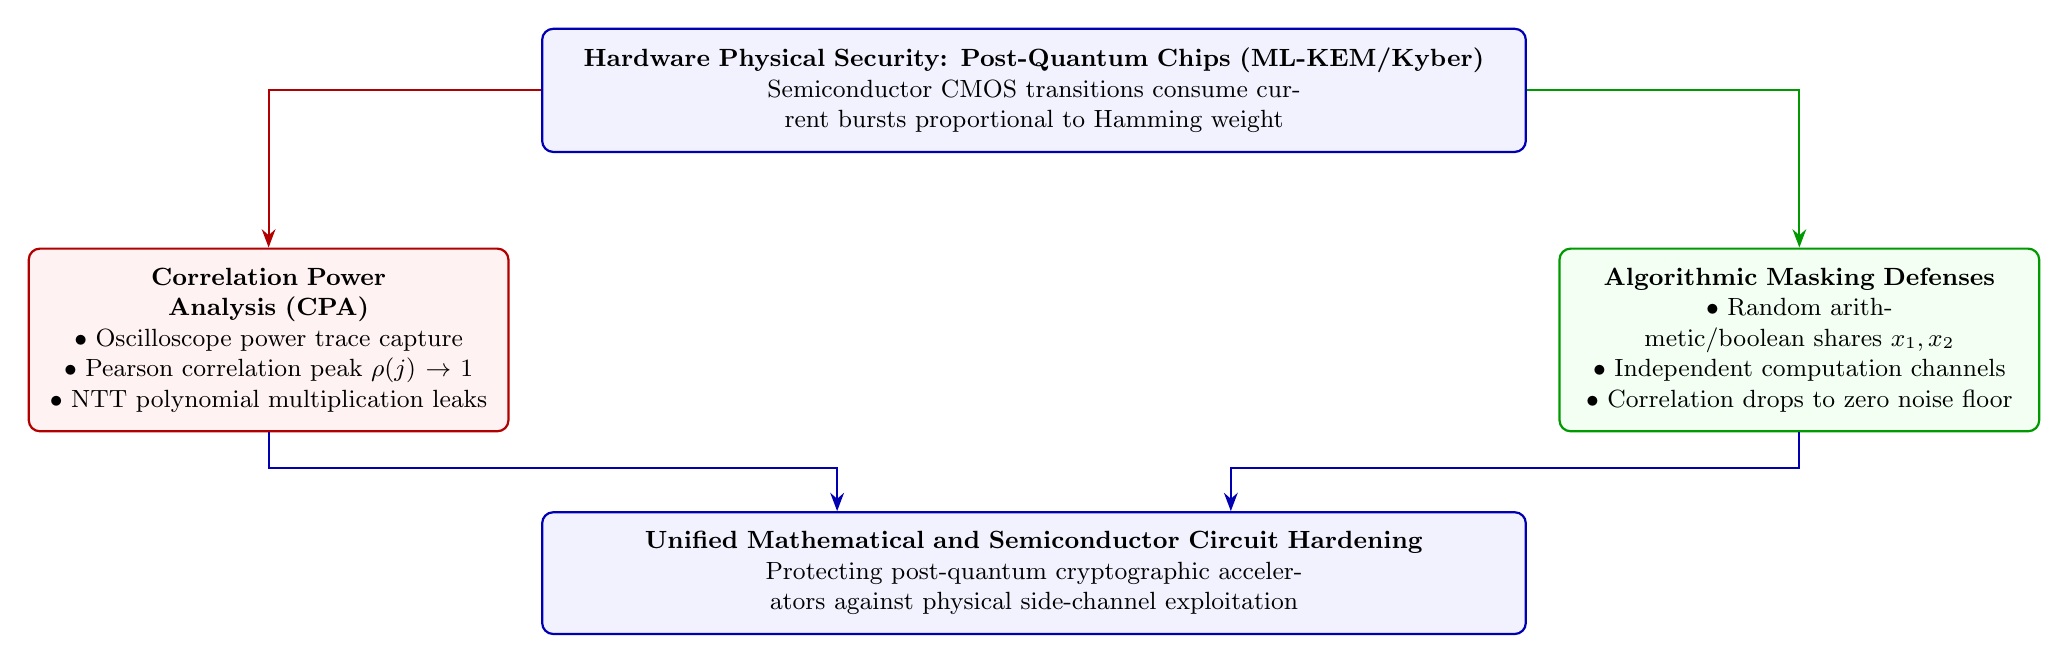
\begin{tikzpicture}[
    font=\small,
    >=Stealth,
    node distance=1.2cm,
    block/.style={rectangle, draw=blue!70!black, fill=blue!5, rounded corners=4pt, thick, align=center, inner sep=7pt},
    alertblock/.style={rectangle, draw=red!70!black, fill=red!5, rounded corners=4pt, thick, align=center, inner sep=7pt},
    greenblock/.style={rectangle, draw=green!60!black, fill=green!5, rounded corners=4pt, thick, align=center, inner sep=7pt},
    amberblock/.style={rectangle, draw=orange!80!black, fill=orange!5, rounded corners=4pt, thick, align=center, inner sep=7pt}
]

\node[block, text width=12cm] (top) {\textbf{Hardware Physical Security: Post-Quantum Chips (ML-KEM/Kyber)}\\Semiconductor CMOS transitions consume current bursts proportional to Hamming weight};

\node[alertblock, below left=1.2cm and 0.4cm of top, text width=5.6cm] (cpa) {\textbf{Correlation Power Analysis (CPA)}\\$\bullet$ Oscilloscope power trace capture\\$\bullet$ Pearson correlation peak $\rho(j) \to 1$\\$\bullet$ NTT polynomial multiplication leaks};

\node[greenblock, below right=1.2cm and 0.4cm of top, text width=5.6cm] (masking) {\textbf{Algorithmic Masking Defenses}\\$\bullet$ Random arithmetic/boolean shares $x_1, x_2$\\$\bullet$ Independent computation channels\\$\bullet$ Correlation drops to zero noise floor};

\node[block, below=1.0cm of $(cpa.south)!0.5!(masking.south)$, text width=12cm] (bottom) {\textbf{Unified Mathematical and Semiconductor Circuit Hardening}\\Protecting post-quantum cryptographic accelerators against physical side-channel exploitation};

\draw[->, thick, red!70!black] (top) -| (cpa);
\draw[->, thick, green!60!black] (top) -| (masking);
\draw[->, thick, blue!70!black] (cpa.south) -- ++(0,-0.45) -| ([xshift=-2.5cm]bottom.north);
\draw[->, thick, blue!70!black] (masking.south) -- ++(0,-0.45) -| ([xshift=2.5cm]bottom.north);

\end{tikzpicture}
\end{document}
